\chapter{函数最优逼近}
\entry \emph{逼近}与\emph{插值}的区别:插值要求通过数据点,逼近则不要求;逼近追求\emph{在给定的函数形式下}整个区间或所有值点
上的\emph{总体误差}最小。

\entry 用\emph{多项式}逼近:便于计算;便于用其做微积分。

\section{内积、范数与正交多项式}
\define \setkey{函数在点集上的内积}{函数内积(点集)}:设$f(x)$,$g(x)$在$X=\{x_1,x_2,
\ldots,x_m\}$上有定义,并有相应的$m$个\emph{权系数}$\omega_i$,则定义
\[(f,g)=\sum_{i=1}^m\omega_if(x_i)g(x_i)\]
为$f$与$g$在$X$上关于权系数$\omega_i$的\emph{内积}。

\define \setkey{函数在区间上的内积}{函数内积(区间)}:设$f,g\in C[a,b]$,$\omega(x)
\in C[a,b]$为权系数,定义
\[(f,g)=\int_a^b\omega(x)f(x)g(x)\di x\]
为$f$与$g$在$[a,b]$上关于$\omega(x)$的内积。

\entry 对权系数的要求:$\omega_i>0$或$\omega(x)\geq0$。常取$\omega_i=1$及
$\omega(x)\equiv1$。

\trm 内积的性质
\footnote{该四条性质对一切「内积空间」都是成立的。}
:
\begin{enumerate}\tl
    \item 对称性:$(f,g)=(g,f)$。
    \item 齐性:对任意的常数$\alpha$,$(\alpha f,g)=(f,\alpha g)=\alpha\cdot(f,g)$。
    \item 可加性:$(f+h,g)=(f,g)+(h,g)$。
    \item 正定性:$(f,f)\geq0$,且仅当$f\equiv0$时$(f,f)=0$。
\end{enumerate}

\define \setkey{函数在点集或区间上的范数}{函数范数}:对点集$X$上所有函数$f$,或对区间上
所有连续函数$f\in C[a,b]$定义运算$\|f\|$,满足:
\begin{enumerate}\tl
    \item (正定性)$\|f\|\geq0$,且仅当$f\equiv0$时$\|f\|=0$。
    \item (线性)对任意的常数$\alpha$,$\|\alpha f\|=|\alpha|\cdot\|f\|$。
    \item (三角不等式)$\|f+g\|\leq\|f\|+\|g\|$。
\end{enumerate}

\entry 常用范数:
\begin{itemize}\tl
    \item 由函数内积导出的$2$-范数:$\|f(x)\|_2=\sqrt{(f,f)}$。
    \item $1$-范数:$\|f\|_1=\sum\limits_{i=1}^m|f(x_i)|$或$\|f\|_1=\int_a^b|f(x)|\di x$。
    \item $\infty$-范数:$\|f\|_\infty=\max\limits_{1\leq i\leq m}|f(x_i)|$或
    $\|f\|_\infty=\max\limits_{a\leq x\leq b}|f(x)|$。
\end{itemize}

\entry 函数的\key{正交}:
\begin{itemize}\tl
    \item 在权函数$\omega_i$(或$\omega(x)$)下,若$(f,g)=0$,则称两函数关于权函数
    $\omega_i$(或$\omega(x)$)正交,称$f$与$g$为\key{正交函数}。
    \item 设有函数族$\{g_k\}$,若其中各函数$g_0(x),g_1(x),\cdots,g_k(x),\cdots$满足
    $(g_i,g_j)=0\,(i\neq j)$,则称$\{g_k\}$为关于$\omega$\setkey{正交}{正交函数族}的函数族。
    \item 若正交函数族$\{g_k\}$进一步满足$\|g_i(x)\|=1\,(\forall i)$,则称其为一个
    \key{标准正交函数族}。
    \item 若正交函数族$\{g_k\}$中的$g_k(x)$为$k$次多项式,则称$g_0(x),\cdots,g_k(x),
    \cdots$为\key{正交多项式}。
\end{itemize}

\trm \emph{正交多项式基本性质}:各正交多项式之间线性无关
\footnote{证明:利用正交性与正定性。}
。(由此,可用一族正交多项式线性表示各阶多项式。)

\trm 推论 1:对$k<n$,$k$次多项式$P_k(x)$与$n$次\emph{正交多项式} $g_n(x)$正交
\footnote{证明:$P_k(x)$可用$g_0(x),\cdots,g_k(x)$线性表出,进而由$g_k(x)$的正交性推得其与$g_n(x)$正交。}
。

\trm 推论 2:在区间$[a,b]$(连续)或$[\min x_i,\max x_i]$(离散)上,$n$次正交多项式
$g_n(x)$恰有$n$个不同实零点
\footnote{证明思路:有实根\sothat 无偶重根\sothat 均为实根\sothat
无多于$1$重的奇实根。}
。

\trm\label{5-t1} 推论 3:设$g_0(x),g_1(x),\cdots,g_k(x),\cdots$均为\emph{首一\footnotemark 正交多项式},则
\footnotetext{即最高次项系数为 $1$。}
\begin{gather}
g_0(x)=1,\,g_1(x)=x-b_0,\,g_{k+1}(x)=(x-b_x)g_k(x)-c_kg_{k-1}(x)\label{5-e1}\\
b_k=\frac{\beta_k}{\gamma_k},c_k=\frac{\gamma_k}{\gamma_{k-1}},\beta_k=(xg_k,g_k),
\gamma_k=(g_k,g_k).\notag
\end{gather}
称以上公式为正交多项式的\key{三项递推关系}
\footnote{证明略去,参见李乃成、梅立泉《数值分析》第146页性质5.1.3的证明。会用即可。}。

\entry \key{Legendre 多项式}:在区间$[-1,1]$上,定义为
\begin{equation}
P_k(x)=\frac1{2^k\cdot k!}\frac{\di^k}{\di x^k}\left[(x^2-1)^k\right].\quad(k=0,
1,2,\ldots)
\end{equation}
其关于权函数$\omega(x)\equiv1$正交。最高次项系数为$\alpha_k=\frac{(2k)!}{2^k\cdot
(k!)}$。

\entry 其他常见正交多项式:
\begin{itemize}\tl
    \item \key{Laguerre 多项式}:$L_k(x)=\e^x\frac{\di(x^k\e^{-x})}{\di x^k}$,正交区间
    为$[0,+\infty)$,权函数为$\omega(x)=\e^{-x}$。
    \item \key{Hermite 多项式}:$H_k(x)=(-1)^k\e^{x^2}\frac{\di^k\e^{-x^2}}{\di x^k}$,
    正交区间为$(-\infty,+\infty)$,权函数为$\omega(x)=\e^{-x^2}$。
    \item \key{Cheybyshev 多项式}:$T_k(x)=\cos(k\arccos x)$,正交区间为$[-1,1]$,权函数
    为$\omega(x)=\frac1{\sqrt{1-x^2}}$。
\end{itemize}

\section{最优平方逼近}
\entry 最优平方逼近:对函数$f(x)$,构造逼近多项式$p(x)$,使按$2$-范数度量得到的误差之平方$S=
\|p-f\|_2^2$最小
\footnote{取平方是因为 2-范数中的根号不易处理。更常见的说法是「均方误差(MSE)最小」,此概念在统计学、机器学习等领域更为常见。}
。

\entry 为系统地实现这一构造过程,常用一多项式函数族$\{\vphi_k(x)\}$表出$p(x)$:
\begin{equation}\label{5-e2}
    p(x)=c_0\vphi_0(x)+\cdots+c_n\vphi_n(x),
\end{equation}
从而问题需落实为:
\begin{enumerate}\tl
    \item 多项式族$\{\vphi_k(x)\}$的选取或导出;
    \item 系数$c_k$的求解。
\end{enumerate}

\define 若$f$为\emph{列表函数},则称逼近其的$p(x)$为\key{最小二乘拟合多项式},误差表达式为
\[\|p-f\|_2=\sqrt{\sum_{i=1}^m\omega_i\biggl[p(x_i)-y_i\biggr]^2}.\]

\define 若$f$为连续函数,则称逼近其的$p(x)$为\key{最优平方逼近多项式},误差为
\[\|p-f\|_2=\sqrt{\int_a^b(p-f)^2\di x}.\]

\entry \key{正规方程组}:按定义将$S=\|p-f\|_2^2$拆开:
\begin{gather}
S=(p-f,p-f)=(p,p)-2(p,f)+(f,f)\notag\\
S=\sum_{i=0}^nc_i\sum_{j=0}^nc_j(\vphi_i,\vphi_j)-2\sum_{i=0}^nc_i(\vphi_i,f)+
(f,f).\label{5-e3}
\end{gather}
视$S$为系数$c_0,\cdots,c_n$的函数,欲使$S$达到极小值,令
\[\frac{\del S}{\del c_k}=2\sum_{i=0}^nc_j(\vphi_k,\vphi_j)-2(\vphi_k,f)=0\]
从而得用于求解系数$c_i$的\key{正规方程组}
\begin{equation}
\sum_{i=0}^nc_j(\vphi_k,\vphi_j)=(\vphi_k,f)
\end{equation}
或
\begin{equation}\label{5-e4}
\begin{pmatrix}(\vphi_0,\vphi_0)&(\vphi_0,\vphi_1)&\cdots&(\vphi_0,\vphi_n)\\
(\vphi_1,\vphi_0)&(\vphi_1,\vphi_1)&\cdots&(\vphi_1,\vphi_n)\\
\vdots&\vdots&\ddots&\vdots\\
(\vphi_n,\vphi_0)&(\vphi_n,\vphi_1)&\cdots&(\vphi_n,\vphi_n)\end{pmatrix}
\begin{pmatrix}c_0\\c_1\\\vdots\\c_n\end{pmatrix}=
\begin{pmatrix}(\vphi_0,f)\\(\vphi_1,f)\\\vdots\\(\vphi_n,f)\end{pmatrix}.
\end{equation}

\entry 正规方程组中,系数矩阵为\emph{对称正定阵},有唯一解。故最优平方逼近的结果存在且唯一。

\entry 正规方程组可改写为
\begin{equation}
(\vphi_k,p-f)=0\quad(k=0,1,\ldots,n).
\end{equation}
意义:误差向量$(p-f)$在由有限个向量$\vphi_k$张成的空间下无投影,控制「低维误差」。

\entry 正规方程组解法 1:选取一组线性无关、内积易求的简单函数作 $\{\vphi_k\}$(常用 $1,x,x^2,\cdots$),计算内积,代入正规方程组直接求解(在问题简单时最为便捷)。

\entry 正规方程组解法 2:选取 $\{\vphi_k\}$ 为一组正交多项式,则正规方程组简化为
\[(\vphi_k,\vphi_k)c_k=(\vphi_k,f),\]
从而易得$c_k=\frac{(\vphi_k,f)}{(\vphi_k,\vphi_k)}$,进而得逼近多项式为
\begin{equation}\label{5-e4.5}
P(x)=\sum_{k=0}^n\frac{(\vphi_k,f)}{(\vphi_k,\vphi_k)}\vphi_k(x).
\end{equation}

\entry 函数族$\vphi_k(x)$的选取原则:
\begin{enumerate}\tl
    \item 直观性原则:观察$(x_i,y_i)$的分布,选取函数族。
    \item 比较性原则:对不同的函数族,可分别拟合,再比较它们的误差向量孰大孰小。
    \item 根据实际问题背景选择函数族(如对周期性变化的函数,可用三角函数族)。
\end{enumerate}

\entry \emph{离散的正规方程组}(\key{最小二乘法}):记
\begin{gather*}
G=\begin{pmatrix}\vphi_0(x_1)&\vphi_1(x_1)&\cdots&\vphi_n(x_1)\\
\vphi_0(x_2)&\vphi_1(x_2)&\cdots&\vphi_n(x_2)\\
\vdots&\vdots&\ddots&\vdots\\
\vphi_0(x_m)&\vphi_1(x_m)&\cdots&\vphi_n(x_m)\end{pmatrix},\,
W=\diag(\omega_1,\omega_2,\cdots,\omega_m),\\
y=(y_1\,y_2\,\cdots\,y_m)^T,\,c=(c_0\,c_2\,\cdots\,c_n)^T,
\end{gather*}
则原正规方程组可化为
\begin{equation}\label{5-e5}
(G^TWG)c=(G^TW)y.
\end{equation}
特别地,若取$\omega_i=1$,则方程进一步简化为
\begin{equation}
G^TGc=G^Ty,
\end{equation}
此即最小二乘方程,具体形式为
\begin{equation}
\begin{pmatrix}\dsum_{i=1}^m1&\dsum_{i=1}^mx_i&\cdots&\dsum_{i=1}^mx_i^n\\
\dsum_{i=1}^mx_i&\dsum_{i=1}^mx_i^2&\cdots&\dsum_{i=1}^mx_i^{n+1}\\
\vdots&\vdots&\ddots&\vdots\\
\dsum_{i=1}^mx_i^n&\dsum_{i=1}^mx_i^{n+1}&\cdots&\dsum_{i=1}^mx_i^{2n}\end{pmatrix}
\begin{pmatrix}c_0\\c_1\\\vdots\\c_n\end{pmatrix}=
\begin{pmatrix}\dsum_{i=1}^my_i\\\dsum_{i=1}^mx_iy_i\\\vdots\\\dsum_{i=1}^mx_i^ny_i
\end{pmatrix}
\end{equation}

\entry 当$m=n+1$时,最小二乘拟合多项式即插值多项式。

\example 对于若干数据点$(x_i,y_i)$,欲采用$y=b\e^{ax}$进行拟合,其中$a,b$为待定常数;
可对该表达式取对数得
\[\ln y=\ln b+ax\]
再考虑误差函数
\[S(a,b)=\sum_{i=1}^m(\ln b+ax_i-\ln y_i)^2\]
令其对$a$、$b$的偏导数为$0$,即可解出参数值。

\entry 最小二乘拟合/最优平方逼近的\emph{一般方法}:
\begin{enumerate}
    \item 可\emph{自选}一组线性无关的基函数,求解正规方程组(\ref{5-e4})或(\ref{5-e5})。
    一般选取$\vphi_k(x)=x^k$。(难点在列、解方程)
    \item 可利用三项递推关系(\ref{5-e1})\emph{求解一族首一正交多项式}$g_0(x),\cdots,g_n(x)$,
    利用式(\ref{5-e4.5})计算逼近的多项式。(难点在递推、计算内积。)
    \item 可先通过变量代换$x=\frac{a+b}2+\frac{b-a}2t$将区间$[a,b]$替换为$[-1,1]$,
    对变换后的函数$\overline{f}(t)$\emph{用正交的 Legendre 多项式}求出$\overline{P}(t)$,
    最后用$t=\frac{2x-a-b}{b-a}$还原到$P(x)$。(难点在记 Legendre 多项式、展开和计算
    内积。)
\end{enumerate}

\example 求$y=\sqrt x$在$[0,1]$上最优平方逼近一次多项式。(答案:$p(x)=\frac45x+
\frac4{15}$。)
\begin{enumerate}
    \item 用$\vphi_0(x)=1$,$\vphi_1(x)=x$,可列出正规方程组
    \[
    \begin{pmatrix}1&1/2\\1/2&1/3\end{pmatrix}\begin{pmatrix}c_0\\c_1\end{pmatrix}
    =\begin{pmatrix}2/3\\2/5\end{pmatrix}
    \]
    容易求得$c_0=\frac4{15}$,$c_1=\frac45$,从而$p(x)=\frac45x+\frac4{15}$。
    \item 用三项递推式,有$g_0(x)=1$,
    \begin{equation}
    g_1(x)=x-\frac{(x,1)}{(1,1)}=x-\frac12,
    \end{equation}
    故可进一步计算
    \begin{align*}
    (g_1,g_2)&=(x-\frac12,x-\frac12)=\int_0^1(x-\frac12)^2\di x=\frac1{12}\\
    (f,g_0)&=(\sqrt x,1)=\frac23\\
    (f,g_1)&=(\sqrt x,x)-(\sqrt x,\frac12)=\frac25-\frac12\cdot\frac23=
    \frac1{15},
    \end{align*}
    从而有
    \[p(x)=\frac23+\frac{1/15}{1/12}\cdot\left(x-\frac12\right)=\frac45x+\frac4{
    15}.\]
    \item 用 Legendre 多项式求解,为此先作变量代换$x=\frac12+\frac12t$,被插函数变为
    $\overline{f}(t)=\sqrt{\frac{1+t}2}$,进而可用前两个 Legendre 多项式
    \[P_0(t)=1,\,P_1(t)=t\]
    逼近$\overline{f}(t)$。可以计算各个内积为
    \begin{align*}
    (P_0,P_0)&=\int_{-1}^1\di t=2\\
    (P_1,P_1)&=\int_{-1}^1t^2\di t=\frac23\\
    (f,P_0)&=\int_{-1}^1\sqrt{\frac{1+t}2}=\frac{\sqrt2}2\int_{-1}^1\sqrt{1+t}
    \di(1+t)=\frac{\sqrt2}2\cdot\frac23\cdot(2\sqrt2)=\frac43\\
    (f,P_1)&=\int_{-1}^1\sqrt{\frac{1+t}2}=\frac{\sqrt2}2\int_{=1}^1(\sqrt{1+t})%
    ^3\di(1+t)-(f,P_0)\\
    &=\frac{\sqrt2}2\cdot\frac25\cdot(4\sqrt2)-\frac43=\frac4{15}
    \end{align*}
    从而
    \[\overline{p}(t)=\frac{4/3}2+\frac{4/15}{2/3}t=\frac23+\frac25t\]
    回代$t=2x-1$即得$p(x)=\frac45x+\frac4{15}$。
\end{enumerate}

\begin{figure}[htbp]
\small\centering
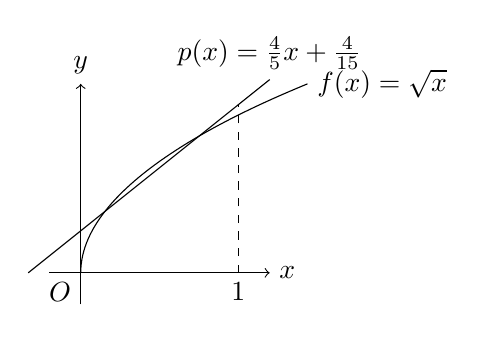
\begin{tikzpicture}[scale=2]
\draw [->] (-0.2,0) -- (1.2,0) node [right] {$x$};
\draw [->] (0,-0.2) -- (0,1.2) node [above] {$y$};
\draw [rotate=90] (0,0) parabola (1.2,-1.44) node [right] {$f(x)=\sqrt x$};
\draw (-1/3,0) -- (1.2,1.227) node [above] {$p(x)=\frac45x+\frac4{15}$};
\node at (0,0) [below left] {$O$};
\draw [dashed] (1,0) node [below] {$1$} -- (1,16/15);
\end{tikzpicture}
\caption{$y=\sqrt x$ 的最优逼近一次多项式示意图}
\end{figure}